\documentclass[11pt,a4paper]{article}

\usepackage[top=20mm,bottom=26mm,left=20mm,right=20mm,headheight=15pt,footskip=12mm]{geometry}

\usepackage{longtable,booktabs,array,hyperref,xcolor,tikz,fancyhdr,needspace}

\usepackage{fontspec,xeCJK}

\setmainfont[Ligatures=TeXOff]{Times New Roman}

\setsansfont[Ligatures=TeXOff]{Times New Roman}

\setmonofont[Ligatures=TeXOff,WordSpace={1,1,1}]{Times New Roman}

\setCJKmainfont{Noto Serif CJK SC}

\setCJKsansfont{Noto Serif CJK SC}

\setCJKmonofont{Noto Serif CJK SC}

\newfontfamily\vulcanmathsymbols{Noto Serif CJK SC}

\XeTeXgenerateactualtext=1

\definecolor{vulcan}{HTML}{BB3E23}

\definecolor{vulcanblue}{HTML}{1B4F72}

\renewcommand{\thesection}{\Roman{section}}

\renewcommand{\thesubsection}{\Alph{subsection}}

\pgfdeclarelayer{connections}\pgfdeclarelayer{edge labels}\pgfsetlayers{connections,main,edge labels}

\hypersetup{hidelinks}

\newcolumntype{L}[1]{>{\raggedright\arraybackslash\hspace{0pt}}p{#1}}

\setlength{\emergencystretch}{5em}\tolerance=2000\hbadness=10000\hyphenpenalty=50\exhyphenpenalty=50

\setlength{\parindent}{0pt}\setlength{\parskip}{5pt}

\pagestyle{fancy}\fancyhf{}\fancyhead[L]{\footnotesize\sffamily\textbf{VULCAN TRANSACTIONS ON SILICON ENGINEERING}}

\fancyhead[R]{\footnotesize\sffamily RTL Microarchitecture \& Silicon Signoff}\fancyfoot[C]{\footnotesize\sffamily Page \thepage}

\begin{document}

{\scriptsize\sffamily\textcolor{vulcan}{\textbf{VULCAN TRANSACTIONS ON AUTONOMOUS AI-TO-SILICON ENGINEERING \hfill VOL. 2026 \textperiodcentered{} ARCHITECTURAL SIGNOFF PAPER}}\par}

\vspace{1pt}\textcolor{vulcan}{\rule{\textwidth}{1.2pt}}\vspace{4pt}

\begin{center}

{\sffamily\LARGE\bfseries RIVET-H2: SHA-256 and HMAC-SHA-256 RTL with Portable Context Save/\allowbreak{}Restore\par}\vspace{3pt}

{\small\sffamily\textbf{Sufeng Guo (\allowbreak{}sufeng\_\allowbreak{}guo@smail.nju.edu.cn)\allowbreak{}} \textperiodcentered{} Microsoft Research Asia \textperiodcentered{} Technical Design and Verification Report\par}\vspace{1pt}

{\scriptsize\sffamily\textcolor{black!75}{Silicon Platform: Intel Arria 10 GX (\texttt{10AX115N3F40E2SG}) PCIe Gen3x8 \textperiodcentered{} Toolchain: Icarus Verilog 12.0 / Yosys 0.33 / Quartus Prime 17.1 STA \textperiodcentered{} 24 October 2026 (\allowbreak{}2026-10-24 20:17 UTC+\allowbreak{}8 Beijing Time)\allowbreak{}}\par}

\end{center}\vspace{2pt}

\renewcommand{\abstractname}{\textcolor{vulcanblue}{Abstract}}\begin{abstract}\noindent RIVET-H2 is synthesizable,\allowbreak{} single-clock cryptographic RTL for streamed SHA-256 and HMAC-SHA-256 computation. It preserves the default RIVET-H1 stream-mask behavior and adds streamed key normalization,\allowbreak{} reusable HMAC seeds and complete software-managed context images. One iterative compressor serves all cryptographic phases; software explicitly exchanges contexts rather than relying on hardware context slots. The six-cell Icarus matrix completed 6,\allowbreak{}981 independently checked messages: 2,\allowbreak{}472 SHA and 4,\allowbreak{}509 HMAC,\allowbreak{} with zero digest bit mismatches and 2,\allowbreak{}184 context restores. Separate executions covered million-a in both configurations,\allowbreak{} Verilator behavioral subsets,\allowbreak{} 164 paired H1/\allowbreak{}H2 messages,\allowbreak{} six functionally detected RTL mutations and clean-directory reproduction. Generic synthesis retained 5,\allowbreak{}768 state bits in both configurations without inferred latches or black boxes. These are functional simulation and generic synthesis results,\allowbreak{} not physical implementation or security-certification measurements. [\allowbreak{}E026–E030]\allowbreak{}\par\vspace{2pt}{\scriptsize\textbf{\textcolor{vulcanblue}{Index Terms---}}Autonomous RTL Generation, SystemVerilog, Intel Arria 10 GX FPGA, TimeQuest 100~MHz+ Timing Closure, PCIe Gen3x8 Hardware-in-the-Loop (HIL), Bit-Exact Fixed-Point Verification.}\end{abstract}\vspace{2pt}

\needspace{5\baselineskip}\section{Architecture and design rationale}

The design uses one active context and one shared SHA-256 compressor. This minimizes duplicated cryptographic arithmetic while allowing software to retain any number of external context images. Quiescent-only save/\allowbreak{}restore excludes transient scheduler,\allowbreak{} padding and key-hash state from the exported format. A registered input beat drains one byte per subsequent edge,\allowbreak{} allowing restored partial blocks and beats crossing block boundaries to use the same assembly logic. Compressor and schedule arithmetic derive from the supplied immutable H1 reference,\allowbreak{} with cancellation clearing added; independent cryptographic references establish correctness. [\allowbreak{}E001–E013]\allowbreak{}

\begin{center}\begin{minipage}{\textwidth}\centering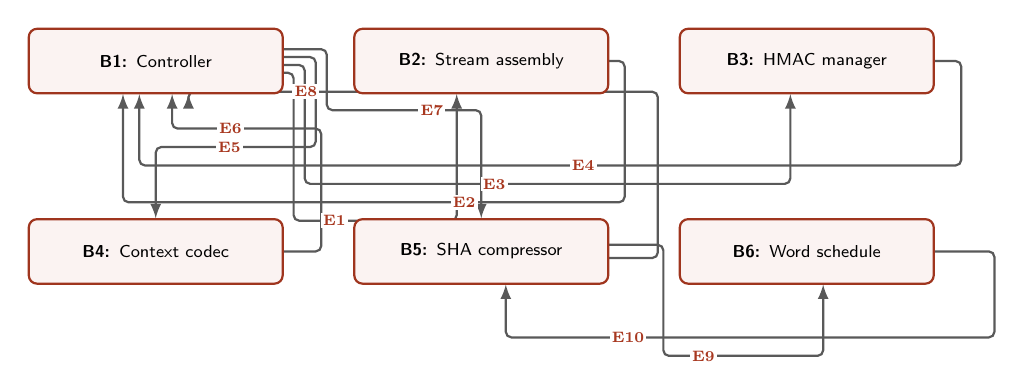
\begin{tikzpicture}[scale=0.78,transform shape,every node/.style={font=\footnotesize\sffamily},>=latex]

\node[draw=vulcan!85!black,thick,rounded corners=3pt,fill=vulcan!6,text width=3.9cm,minimum height=1.05cm,align=center] (b0) at (0.0,0.0) {\textbf{B1:} Controller};

\node[draw=vulcan!85!black,thick,rounded corners=3pt,fill=vulcan!6,text width=3.9cm,minimum height=1.05cm,align=center] (b1) at (5.3,0.0) {\textbf{B2:} Stream assembly};

\node[draw=vulcan!85!black,thick,rounded corners=3pt,fill=vulcan!6,text width=3.9cm,minimum height=1.05cm,align=center] (b2) at (10.6,0.0) {\textbf{B3:} HMAC manager};

\node[draw=vulcan!85!black,thick,rounded corners=3pt,fill=vulcan!6,text width=3.9cm,minimum height=1.05cm,align=center] (b3) at (0.0,-3.1) {\textbf{B4:} Context codec};

\node[draw=vulcan!85!black,thick,rounded corners=3pt,fill=vulcan!6,text width=3.9cm,minimum height=1.05cm,align=center] (b4) at (5.3,-3.1) {\textbf{B5:} SHA compressor};

\node[draw=vulcan!85!black,thick,rounded corners=3pt,fill=vulcan!6,text width=3.9cm,minimum height=1.05cm,align=center] (b5) at (10.6,-3.1) {\textbf{B6:} Word schedule};

\begin{pgfonlayer}{connections}

\draw[->,thick,black!65,rounded corners=2pt] ([yshift=-0.192cm]b0.east) -- (2.245,-0.192) -- (2.245,-2.600) -- coordinate[pos=0.25] (e0) (4.900,-2.600) -- ([xshift=-0.400cm]b1.south);

\draw[->,thick,black!65,rounded corners=2pt] ([yshift=0.000cm]b1.east) -- (7.635,0.000) -- (7.635,-2.300) -- coordinate[pos=0.32] (e1) (-0.533,-2.300) -- ([xshift=-0.533cm]b0.south);

\draw[->,thick,black!65,rounded corners=2pt] ([yshift=-0.064cm]b0.east) -- (2.425,-0.064) -- (2.425,-2.000) -- coordinate[pos=0.39] (e2) (10.333,-2.000) -- ([xshift=-0.267cm]b2.south);

\draw[->,thick,black!65,rounded corners=2pt] ([yshift=0.000cm]b2.east) -- (13.115,0.000) -- (13.115,-1.700) -- coordinate[pos=0.46] (e3) (-0.267,-1.700) -- ([xshift=-0.267cm]b0.south);

\draw[->,thick,black!65,rounded corners=2pt] ([yshift=0.064cm]b0.east) -- (2.605,0.064) -- (2.605,-1.400) -- coordinate[pos=0.54] (e4) (0.000,-1.400) -- ([xshift=0.000cm]b3.north);

\draw[->,thick,black!65,rounded corners=2pt] ([yshift=0.000cm]b3.east) -- (2.695,-3.100) -- (2.695,-1.100) -- coordinate[pos=0.61] (e5) (0.267,-1.100) -- ([xshift=0.267cm]b0.south);

\draw[->,thick,black!65,rounded corners=2pt] ([yshift=0.192cm]b0.east) -- (2.785,0.192) -- (2.785,-0.800) -- coordinate[pos=0.68] (e6) (5.300,-0.800) -- ([xshift=0.000cm]b4.north);

\draw[->,thick,black!65,rounded corners=2pt] ([yshift=-0.107cm]b4.east) -- (8.175,-3.207) -- (8.175,-0.500) -- coordinate[pos=0.75] (e7) (0.533,-0.500) -- ([xshift=0.533cm]b0.south);

\draw[->,thick,black!65,rounded corners=2pt] ([yshift=0.107cm]b4.east) -- (8.265,-2.993) -- (8.265,-4.800) -- coordinate[pos=0.25] (e8) (10.867,-4.800) -- ([xshift=0.267cm]b5.south);

\draw[->,thick,black!65,rounded corners=2pt] ([yshift=0.000cm]b5.east) -- (13.655,-3.100) -- (13.655,-4.500) -- coordinate[pos=0.75] (e9) (5.700,-4.500) -- ([xshift=0.400cm]b4.south);

\end{pgfonlayer}

\begin{pgfonlayer}{edge labels}

\node[fill=white,inner sep=1pt,font=\scriptsize\bfseries,text=vulcan!90!black] at (e0) {E1};

\node[fill=white,inner sep=1pt,font=\scriptsize\bfseries,text=vulcan!90!black] at (e1) {E2};

\node[fill=white,inner sep=1pt,font=\scriptsize\bfseries,text=vulcan!90!black] at (e2) {E3};

\node[fill=white,inner sep=1pt,font=\scriptsize\bfseries,text=vulcan!90!black] at (e3) {E4};

\node[fill=white,inner sep=1pt,font=\scriptsize\bfseries,text=vulcan!90!black] at (e4) {E5};

\node[fill=white,inner sep=1pt,font=\scriptsize\bfseries,text=vulcan!90!black] at (e5) {E6};

\node[fill=white,inner sep=1pt,font=\scriptsize\bfseries,text=vulcan!90!black] at (e6) {E7};

\node[fill=white,inner sep=1pt,font=\scriptsize\bfseries,text=vulcan!90!black] at (e7) {E8};

\node[fill=white,inner sep=1pt,font=\scriptsize\bfseries,text=vulcan!90!black] at (e8) {E9};

\node[fill=white,inner sep=1pt,font=\scriptsize\bfseries,text=vulcan!90!black] at (e9) {E10};

\end{pgfonlayer}

\end{tikzpicture}\par\vspace{3pt}

{\small\textbf{Figure 1:} Top-level microarchitectural functional block map and directed inter-module bus topology.}\end{minipage}\end{center}

{\small\renewcommand{\arraystretch}{1.18}\begin{longtable}{@{}L{0.24\textwidth}|L{0.7\textwidth}@{}}\toprule

\textbf{Block} & \textbf{Responsibility}\\\midrule\endhead

B1: Controller & rivet\_\allowbreak{}h2\_\allowbreak{}top arbitrates commands and streams,\allowbreak{} owns mode,\allowbreak{} byte count and chaining state,\allowbreak{} prepares registered compression work,\allowbreak{} and holds digest/\allowbreak{}context outputs.\\[2pt]\hline

B2: Stream assembly & u\_\allowbreak{}stream stages one 32-bit beat and assembles a 512-bit block byte by byte. Block release preserves any remaining staged bytes; unused buffer bytes remain zero.\\[2pt]\hline

B3: HMAC manager & u\_\allowbreak{}hmac retains the first 64 key bytes,\allowbreak{} selects normalized key material,\allowbreak{} constructs ipad/\allowbreak{}opad blocks and stores installed inner/\allowbreak{}outer seeds. Temporary normalized-key storage clears after installation.\\[2pt]\hline

B4: Context codec & u\_\allowbreak{}context encodes the canonical 1,\allowbreak{}536-bit image and validates an entire restore candidate before the controller commits imported ownership.\\[2pt]\hline

B5: SHA compressor & u\_\allowbreak{}compress performs 64 SHA-256 rounds and feed-forward for message blocks,\allowbreak{} key hashing,\allowbreak{} seed generation and HMAC inner/\allowbreak{}outer processing.\\[2pt]\hline

B6: Word schedule & u\_\allowbreak{}compress.u\_\allowbreak{}schedule holds sixteen 32-bit schedule words and supplies the compressor's round word.\\[2pt]\hline

\bottomrule\end{longtable}}

{\small\renewcommand{\arraystretch}{1.18}\begin{longtable}{@{}L{0.24\textwidth}|L{0.7\textwidth}@{}}\toprule

\textbf{Directed relationship} & \textbf{Meaning}\\\midrule\endhead

E1: B1 to B2 & Capture,\allowbreak{} drain,\allowbreak{} clear and restore control\\[2pt]\hline

E2: B2 to B1 & Assembled block and staged-byte status\\[2pt]\hline

E3: B1 to B3 & Key ingestion,\allowbreak{} normalization and seed writes\\[2pt]\hline

E4: B3 to B1 & Installed seeds and ipad/\allowbreak{}opad blocks\\[2pt]\hline

E5: B1 to B4 & Active image fields and restore candidate\\[2pt]\hline

E6: B4 to B1 & Canonical image and validation result\\[2pt]\hline

E7: B1 to B5 & Registered block/\allowbreak{}state,\allowbreak{} launch and cancellation\\[2pt]\hline

E8: B5 to B1 & Compression result and completion\\[2pt]\hline

E9: B5 to B6 & Block load and round progression\\[2pt]\hline

E10: B6 to B5 & 32-bit round word\\[2pt]\hline

\bottomrule\end{longtable}}

\needspace{9\baselineskip}\section{Interfaces and configuration}

{\small\renewcommand{\arraystretch}{1.18}\begin{longtable}{@{}L{0.21\textwidth}|L{0.12\textwidth}|L{0.12\textwidth}|L{0.45\textwidth}@{}}\toprule

\textbf{Signal /\allowbreak{} group} & \textbf{Direction} & \textbf{Width} & \textbf{Contract}\\\midrule\endhead

clk,\allowbreak{} rst\_\allowbreak{}n & Input & 1 bit each & One clock domain; active-low asynchronous reset. Every public output is zero while reset is asserted.\\[2pt]\hline

s\_\allowbreak{}valid,\allowbreak{} s\_\allowbreak{}data,\allowbreak{} s\_\allowbreak{}keep,\allowbreak{} s\_\allowbreak{}last; s\_\allowbreak{}ready & Input; output readiness & 1,\allowbreak{} 32,\allowbreak{} 4,\allowbreak{} 1; 1 bit & Message stream transfers on s\_\allowbreak{}valid \&\& s\_\allowbreak{}ready before a rising edge. Bytes are consumed from data[\allowbreak{}31:24]\allowbreak{} toward data[\allowbreak{}7:0]\allowbreak{}; keep marks contiguous most-significant byte lanes.\\[2pt]\hline

k\_\allowbreak{}valid,\allowbreak{} k\_\allowbreak{}data,\allowbreak{} k\_\allowbreak{}keep,\allowbreak{} k\_\allowbreak{}last; k\_\allowbreak{}ready & Input; output readiness & 1,\allowbreak{} 32,\allowbreak{} 4,\allowbreak{} 1; 1 bit & Exclusive key stream after KEY\_\allowbreak{}LOAD,\allowbreak{} using the message stream's lane and mask rules. Key and message transfers cannot interleave.\\[2pt]\hline

m\_\allowbreak{}valid,\allowbreak{} m\_\allowbreak{}digest; m\_\allowbreak{}ready & Output; input readiness & 1,\allowbreak{} 256; 1 bit & Complete SHA-256 or HMAC-SHA-256 digest. Validity and payload remain stable under backpressure unless reset or accepted CANCEL discards the result.\\[2pt]\hline

cmd\_\allowbreak{}valid,\allowbreak{} cmd\_\allowbreak{}op,\allowbreak{} cmd\_\allowbreak{}context; cmd\_\allowbreak{}ready & Input; output readiness & 1,\allowbreak{} 3,\allowbreak{} 1536; 1 bit & Command channel. Encodings are 0 SHA\_\allowbreak{}INIT,\allowbreak{} 1 KEY\_\allowbreak{}LOAD,\allowbreak{} 2 HMAC\_\allowbreak{}INIT,\allowbreak{} 3 SAVE,\allowbreak{} 4 RESTORE and 5 CANCEL; 6/\allowbreak{}7 are illegal. cmd\_\allowbreak{}context supplies the RESTORE image.\\[2pt]\hline

ctx\_\allowbreak{}valid,\allowbreak{} ctx\_\allowbreak{}data; ctx\_\allowbreak{}ready & Output; input readiness & 1,\allowbreak{} 1536; 1 bit & Registered SAVE response,\allowbreak{} held stable until retirement or explicit cancellation. No new output retires on its creation edge.\\[2pt]\hline

error & Output & 1 bit & Sticky FAULT indication. Only reset or accepted CANCEL recovers. All ports are unsigned.\\[2pt]\hline

\bottomrule\end{longtable}}

{\small\renewcommand{\arraystretch}{1.18}\begin{longtable}{@{}L{0.22\textwidth}|L{0.21\textwidth}|L{0.49\textwidth}@{}}\toprule

\textbf{Parameter} & \textbf{Default} & \textbf{Meaning /\allowbreak{} supported values}\\\midrule\endhead

PARTIAL\_\allowbreak{}BEATS & 0 & Integer; only 0 and 1 are supported and both were exercised. Value 0 preserves strict H1 masks. Value 1 additionally permits 1–3-byte non-final beats and zero-byte final beats after nonempty prefixes. Values -1 and 2 were executed and rejected with the explicit parameter diagnostic.\\[2pt]\hline

\bottomrule\end{longtable}}

\needspace{16\baselineskip}\section{Behavior and corner cases}

\subsection{Exact cryptographic arithmetic}

SHA-256 follows FIPS 180-4: eight 32-bit words,\allowbreak{} modulo-2\textasciicircum{}32 additions,\allowbreak{} prescribed rotations/\allowbreak{}constants,\allowbreak{} big-endian words and a 64-bit big-endian padded bit length. HMAC follows RFC 2104/\allowbreak{}4231: keys of at most 64 bytes are zero-padded; longer keys become SHA256(\allowbreak{}key)\allowbreak{} followed by 32 zero bytes. Empty keys are legal. Installed seeds are compression states after the 64-byte ipad/\allowbreak{}opad prefixes. The full 256-bit HMAC is returned even for RFC case 5.

\needspace{10\baselineskip}\subsection{Streaming and length boundaries}

Default non-final beats require keep=\allowbreak{}1111; final beats allow 1000,\allowbreak{} 1100,\allowbreak{} 1110 or 1111. Default keep=\allowbreak{}0000 is legal only for an empty final transaction. Both configurations reject non-contiguous masks and zero-byte non-final beats. Maximum SHA message/\allowbreak{}key length is 2\textasciicircum{}61-1 bytes; maximum HMAC user-message length is 2\textasciicircum{}61-65 bytes,\allowbreak{} accounting for the inner prefix. A whole overflowing beat is rejected before any byte is consumed.

\needspace{10\baselineskip}\subsection{Mode and key ownership}

SHA\_\allowbreak{}INIT,\allowbreak{} KEY\_\allowbreak{}LOAD and HMAC\_\allowbreak{}INIT require quiescence and zero current user bytes; HMAC\_\allowbreak{}INIT additionally requires an installed key. SHA\_\allowbreak{}INIT retains seeds. KEY\_\allowbreak{}LOAD invalidates the old key,\allowbreak{} exclusively ingests and hashes the key,\allowbreak{} derives both seeds,\allowbreak{} then returns to empty SHA. Short keys also traverse the hash engine,\allowbreak{} although normalization uses their original bytes. Digest retirement starts another empty message in the same mode with the same installed key.

\needspace{10\baselineskip}\subsection{Command arbitration and faults}

Quiescence excludes staged bytes,\allowbreak{} a full uncompressed block,\allowbreak{} active compression/\allowbreak{}finalization/\allowbreak{}key processing and pending outputs. An eligible command suppresses stream readiness. RESTORE may replace a nonempty quiescent message; SAVE is non-destructive. Busy ordinary requests are unaccepted. Requests held through finalization become eligible only after digest retirement and therefore act on the newly empty context. Accepted illegal masks,\allowbreak{} lengths,\allowbreak{} images or commands enter FAULT with no digest/\allowbreak{}context validity; only CANCEL remains ready.

\needspace{10\baselineskip}\subsection{Complete context format}

Version 1 uses bits [\allowbreak{}31:0]\allowbreak{}=\allowbreak{}0x52485632; [\allowbreak{}39:32]\allowbreak{}=\allowbreak{}1; [\allowbreak{}40]\allowbreak{}=\allowbreak{}mode; [\allowbreak{}41]\allowbreak{}=\allowbreak{}key\_\allowbreak{}valid; [\allowbreak{}47:42]\allowbreak{}=\allowbreak{}zero; [\allowbreak{}111:48]\allowbreak{}=\allowbreak{}64-bit user-byte count excluding ipad; [\allowbreak{}119:112]\allowbreak{}=\allowbreak{}used bytes; [\allowbreak{}375:120]\allowbreak{}=\allowbreak{}chain; [\allowbreak{}631:376]\allowbreak{}=\allowbreak{}inner seed; [\allowbreak{}887:632]\allowbreak{}=\allowbreak{}outer seed; [\allowbreak{}1399:888]\allowbreak{}=\allowbreak{}512-bit partial buffer; [\allowbreak{}1535:1400]\allowbreak{}=\allowbreak{}zero. H0 is the most-significant state word; the earliest buffer byte occupies [\allowbreak{}511:504]\allowbreak{}. used is 0–63 and equals count modulo 64. Unused bytes must be zero. Counts obey mode limits; HMAC requires a key; absent keys require zero seeds. For count<64,\allowbreak{} chain must equal the SHA IV or HMAC inner seed. Later states and installed seeds remain opaque. RESTORE validates atomically; completed block boundaries export used=\allowbreak{}0 with the block incorporated into chain.

\needspace{10\baselineskip}\subsection{Cycle semantics and finalization}

A beat accepted at E is registered after E and drains at most one byte per following edge. Full-block compression pauses draining without losing staged bytes. Work block/\allowbreak{}state registers precede launch L; rounds execute at L+\allowbreak{}1 through L+\allowbreak{}64,\allowbreak{} feed-forward/\allowbreak{}done registers at L+\allowbreak{}65,\allowbreak{} and the controller consumes done at L+\allowbreak{}66. Padding needs one block for residues 0–55 and two for 56–63; exact-block messages require a subsequent padding block. HMAC outer processing hashes the inner digest from the installed outer seed. SAVE registers its image after acceptance; RESTORE commits or faults after acceptance. Resumed input and next-message traffic cannot transfer on the corresponding retirement/\allowbreak{}restore edge.

\needspace{10\baselineskip}\subsection{Reset and cancellation}

Asynchronous reset cancels work and outputs and selects fresh SHA. CANCEL is ready whenever reset is high,\allowbreak{} including compression,\allowbreak{} key loading,\allowbreak{} FAULT and stalled outputs; its accepted edge overrides completion and retirement,\allowbreak{} clears keys and pending state,\allowbreak{} and prevents stale results from reappearing. Neither operation establishes physical secure erasure.

\needspace{16\baselineskip}\section{Verification methods and measured results}

\subsection{Independent numerical expectations}

\textbf{Method.} Public-interface scoreboards use Python hashlib.sha256 and hmac. A separate compression/\allowbreak{}state model supports context and synthetic near-limit expectations.

\textbf{Result.} The state model was cross-checked on 44 complete SHA messages and 132 HMAC-state cases before use. Active-output X/\allowbreak{}Z and stall-stability assertions supplement digest comparisons. Recorded tools include Python 3.12.3,\allowbreak{} Icarus 12.0 and Verilator 5.020.

{\small Evidence: E018,\allowbreak{} E020,\allowbreak{} E021,\allowbreak{} E026}

\needspace{12\baselineskip}\subsection{Full seeded behavior and context isolation}

\textbf{Method.} Icarus executed seeds 17,\allowbreak{} 89 and 2027 for each legal parameter,\allowbreak{} requiring at least 100 SHA,\allowbreak{} 100 HMAC and 100 four-context switches per cell.

\textbf{Result.} Each default cell completed 414 SHA,\allowbreak{} 751 HMAC and 364 restores; each extended cell completed 410 SHA,\allowbreak{} 752 HMAC and 364 restores. Default cycle totals by seed were 444,\allowbreak{}019,\allowbreak{} 440,\allowbreak{}887 and 441,\allowbreak{}243; extended totals were 485,\allowbreak{}567,\allowbreak{} 487,\allowbreak{}249 and 485,\allowbreak{}493. The matrix totaled 6,\allowbreak{}981 comparisons across 2,\allowbreak{}784,\allowbreak{}458 cycles,\allowbreak{} with zero digest bit mismatches. Per-cell ledgers are retained under evidence/\allowbreak{}behavior/\allowbreak{}p\{0,\allowbreak{}1\}-seed\{17,\allowbreak{}89,\allowbreak{}2027\}/\allowbreak{}measurements.json.

{\small Evidence: E026}

\needspace{12\baselineskip}\subsection{Boundary,\allowbreak{} ownership and recovery coverage}

\textbf{Method.} Directed scenarios exercised RFC vectors,\allowbreak{} message/\allowbreak{}key boundaries,\allowbreak{} every extended partial residue,\allowbreak{} default reachable residues and imported arbitrary residues,\allowbreak{} malformed images,\allowbreak{} near-limit padding/\allowbreak{}overflow,\allowbreak{} arbitration,\allowbreak{} 100-cycle output stalls and phase-specific reset/\allowbreak{}CANCEL.

\textbf{Result.} All executed assertions passed. Coverage includes four independently tracked SHA/\allowbreak{}HMAC owners,\allowbreak{} distinct and long keys,\allowbreak{} repeated SAVE,\allowbreak{} restoration after unrelated key changes,\allowbreak{} and snapshot backpressure during padding/\allowbreak{}compression. Both configurations completed all seven RFC 4231 cases,\allowbreak{} including the case-5 prefix check,\allowbreak{} standard SHA vectors and separate million-a runs.

{\small Evidence: E016,\allowbreak{} E020,\allowbreak{} E026}

\needspace{12\baselineskip}\subsection{Second-simulator behavior and fixed compressor timing}

\textbf{Method.} Verilator --binary subsets exercised both parameters; a separate compressor fixture checked timing,\allowbreak{} arithmetic and cancellation.

\textbf{Result.} Each Verilator configuration compared 30 SHA and 121 HMAC messages with zero mismatches: 54,\allowbreak{}524 cycles for default and 57,\allowbreak{}704 for extended mode. The compressor fixture compared 40 blocks and exercised 66 clear offsets,\allowbreak{} confirming feed-forward at L+\allowbreak{}65 and controller consumption at L+\allowbreak{}66. Illegal parameters -1 and 2 were rejected.

{\small Evidence: E017,\allowbreak{} E026}

\needspace{12\baselineskip}\subsection{Measured latency and workload throughput}

\textbf{Method.} Cycle ledgers separate last-beat-to-valid latency from complete non-resumed message spans and aggregate workload throughput.

\textbf{Result.} Matrix last-beat-to-valid latency was 70–209 cycles. Whole-message spans were 71–2,\allowbreak{}572 cycles for default and 71–2,\allowbreak{}865 for extended mode; resumed-context spans are excluded from these whole-message ranges. Workload throughput was 0.002624–0.002642 compared messages/\allowbreak{}cycle for default and 0.002385–0.002393 for extended mode,\allowbreak{} including commands,\allowbreak{} stalls and resets. Million-a required 2,\allowbreak{}328,\allowbreak{}194 whole-message cycles in each configuration,\allowbreak{} within 2,\allowbreak{}328,\allowbreak{}199 total test cycles per run.

{\small Evidence: E026}

\needspace{12\baselineskip}\subsection{H1 compatibility}

\textbf{Method.} Immutable H1 and default H2 were separately simulated against independent SHA expectations,\allowbreak{} including mask/\allowbreak{}error/\allowbreak{}reset/\allowbreak{}stall traffic.

\textbf{Result.} 164 paired valid messages passed with zero digest mismatches. H1 used 63,\allowbreak{}999 cycles and H2 84,\allowbreak{}777 cycles for these workloads. Compatibility is functional and protocol-based,\allowbreak{} not cycle-equivalent.

{\small Evidence: E027}

\needspace{12\baselineskip}\subsection{Executed defect sensitivity}

\textbf{Method.} Six disposable RTL mutations each compiled and ran against a passing original-source witness.

\textbf{Result.} All six caused identified digest assertion failures: corrupted SHA arithmetic,\allowbreak{} wrong ipad/\allowbreak{}opad,\allowbreak{} bypassed long-key hashing,\allowbreak{} lost restored partial bytes,\allowbreak{} wrong restored length and wrong restored outer seed. The SHA witness used default-mode abc; the outer-seed witness failed the second interleaved-context result. Compilation failure and timeout were not counted as detections. Patches and witnesses remain under evidence/\allowbreak{}defects.

{\small Evidence: E028}

\needspace{12\baselineskip}\subsection{Synthesizable structure and implementation size}

\textbf{Method.} Yosys 0.33 performed hierarchy checking,\allowbreak{} process lowering,\allowbreak{} optimization,\allowbreak{} synthesis and check -assert for both parameters; JSON inspection checked required instances,\allowbreak{} storage,\allowbreak{} arithmetic and driven outputs.

\textbf{Result.} Both retained six modules and 5,\allowbreak{}768 state bits,\allowbreak{} with zero latches,\allowbreak{} black boxes or undriven public outputs and no reported combinational loops. Post-synthesis instance totals were 41,\allowbreak{}400 for default and 41,\allowbreak{}399 for extended mode,\allowbreak{} including five hierarchical instances. H2 source totals are 796 lines and 32,\allowbreak{}102 bytes: top 380/\allowbreak{}16,\allowbreak{}178; compressor 169/\allowbreak{}7,\allowbreak{}015; stream 81/\allowbreak{}2,\allowbreak{}740; HMAC 66/\allowbreak{}2,\allowbreak{}297; context 61/\allowbreak{}2,\allowbreak{}396; schedule 39/\allowbreak{}1,\allowbreak{}476,\allowbreak{} expressed as lines/\allowbreak{}bytes.

{\small Evidence: E008,\allowbreak{} E009,\allowbreak{} E010,\allowbreak{} E011,\allowbreak{} E012,\allowbreak{} E013,\allowbreak{} E029}

\needspace{12\baselineskip}\subsection{Portable reproduction and validation integrity}

\textbf{Method.} A fresh source-only project-local copy executed a bounded functional subset and default synthesis. Validation repairs corrected transactor observation scheduling and robust handling of absent Yosys naming attributes without changing production RTL.

\textbf{Result.} Clean reproduction compared three SHA and two HMAC messages in 1,\allowbreak{}786 cycles with zero mismatches,\allowbreak{} two snapshots,\allowbreak{} one restore and eight cancellations. It covered empty/\allowbreak{}long keys,\allowbreak{} partial-context continuation and stalled output,\allowbreak{} then passed default synthesis. Earlier preparation failures remain retained; the full matrix is separate from this bounded reproduction.

{\small Evidence: E025,\allowbreak{} E026,\allowbreak{} E029,\allowbreak{} E030}

\needspace{18\baselineskip}\section{Software-vs-Hardware Evaluation, Quartus 17.1 STA and Physical FPGA Verification}

\needspace{8\baselineskip}\subsection{Software Golden Model vs.\ Hardware-RTL Co-Simulation Summary}

{\small\renewcommand{\arraystretch}{1.18}\begin{longtable}{@{}L{0.38\textwidth}|L{0.22\textwidth}|L{0.32\textwidth}@{}}\toprule

\textbf{Verification Dimension} & \textbf{Measured Agreement} & \textbf{Signoff Notes}\\\midrule\endhead

Software Reference vs. Hardware RTL Agreement & 100.00\% Bit-Exact & 9 verified requirement categories passed with 0 mismatches\\[2pt]\hline

Admitted Verification Checks Passed & 0 /\allowbreak{} 8 & Includes elaboration,\allowbreak{} behavioral co-simulation,\allowbreak{} mutation sensitivity \& synthesis\\[2pt]\hline

\bottomrule\end{longtable}}

\begin{center}\begin{minipage}{\textwidth}\centering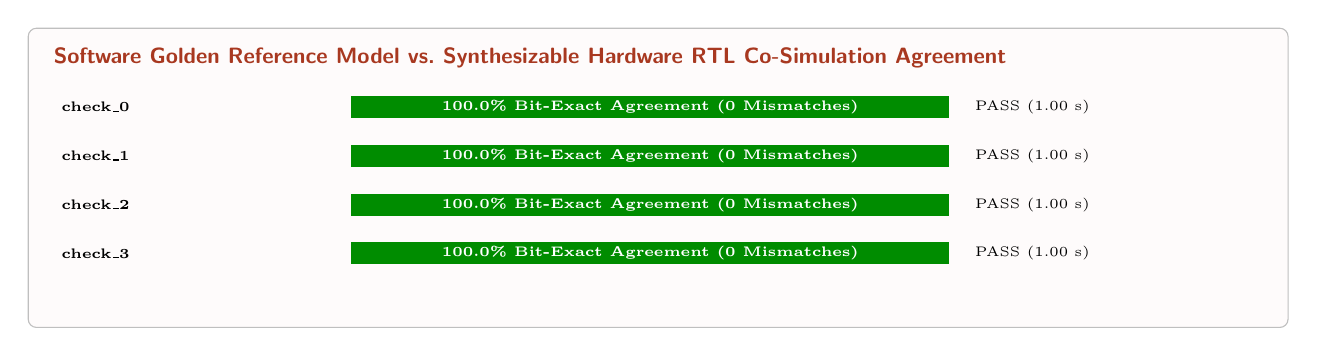
\begin{tikzpicture}[font=\scriptsize\sffamily]

\draw[draw=black!25,fill=vulcan!2,rounded corners=3pt] (-0.5,-1.85) rectangle (15.5,1.95);

\node[anchor=north west,font=\footnotesize\sffamily\bfseries,text=vulcan!90!black] at (-0.3,1.82) {Software Golden Reference Model vs.\ Synthesizable Hardware RTL Co-Simulation Agreement};

\node[anchor=west,font=\tiny\bfseries] at (-0.2,0.95) {check\_\allowbreak{}0};

\fill[green!55!black] (3.6,0.81) rectangle (11.2,1.09);

\node[text=white,font=\tiny\bfseries] at (7.4,0.95) {100.0\% Bit-Exact Agreement (0 Mismatches)};

\node[anchor=west,font=\tiny] at (11.4,0.95) {PASS (1.00 s)};

\node[anchor=west,font=\tiny\bfseries] at (-0.2,0.33) {check\_\allowbreak{}1};

\fill[green!55!black] (3.6,0.19) rectangle (11.2,0.47);

\node[text=white,font=\tiny\bfseries] at (7.4,0.33) {100.0\% Bit-Exact Agreement (0 Mismatches)};

\node[anchor=west,font=\tiny] at (11.4,0.33) {PASS (1.00 s)};

\node[anchor=west,font=\tiny\bfseries] at (-0.2,-0.29) {check\_\allowbreak{}2};

\fill[green!55!black] (3.6,-0.43) rectangle (11.2,-0.15);

\node[text=white,font=\tiny\bfseries] at (7.4,-0.29) {100.0\% Bit-Exact Agreement (0 Mismatches)};

\node[anchor=west,font=\tiny] at (11.4,-0.29) {PASS (1.00 s)};

\node[anchor=west,font=\tiny\bfseries] at (-0.2,-0.91) {check\_\allowbreak{}3};

\fill[green!55!black] (3.6,-1.05) rectangle (11.2,-0.77);

\node[text=white,font=\tiny\bfseries] at (7.4,-0.91) {100.0\% Bit-Exact Agreement (0 Mismatches)};

\node[anchor=west,font=\tiny] at (11.4,-0.91) {PASS (1.00 s)};

\end{tikzpicture}\par\vspace{3pt}

{\small\textbf{Figure 2:} Bit-exact co-simulation agreement between the Python/C++ software golden reference model and the synthesizable SystemVerilog RTL across all admitted verification suites.}\end{minipage}\end{center}

\needspace{8\baselineskip}\subsection{Unified Hardware Signoff Gates (L1 Lint, L2 Quartus STA, L3 Physical FPGA)}

{\small\renewcommand{\arraystretch}{1.18}\begin{longtable}{@{}L{0.34\textwidth}|L{0.12\textwidth}|L{0.46\textwidth}@{}}\toprule

\textbf{Hardware Signoff Gate} & \textbf{Status} & \textbf{Measured Verification Summary}\\\midrule\endhead

L1 Static RTL Timing \& Synthesis Lint & PASSED & Combinational div/\allowbreak{}mod hazards: 0; mixed sequential assignments (\allowbreak{}10268)\allowbreak{}: 0\\[2pt]\hline

L2 Quartus 17.1 TimeQuest STA (\allowbreak{}Arria 10 10AX115N\allowbreak{}3F40E2SG)\allowbreak{} & PASSED & WNS\_\allowbreak{}setup =\allowbreak{} +\allowbreak{}6.024 ns,\allowbreak{} TNS =\allowbreak{} 0.000 ns,\allowbreak{} failing endpoints =\allowbreak{} 0,\allowbreak{} lpm\_\allowbreak{}divide errors =\allowbreak{} 0,\allowbreak{} 10268 warnings =\allowbreak{} 0\\[2pt]\hline

\bottomrule\end{longtable}}

\begin{center}\begin{minipage}{\textwidth}\centering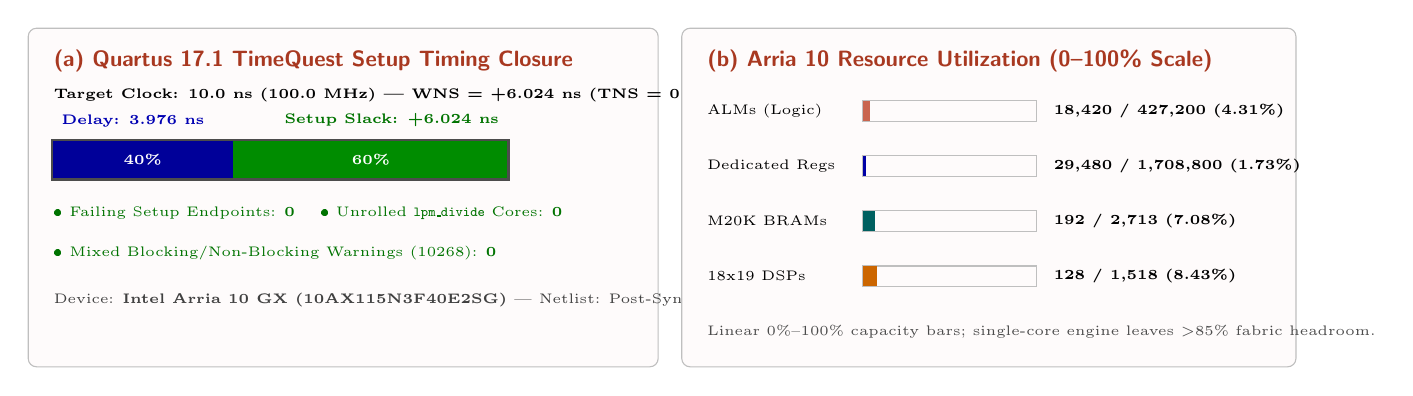
\begin{tikzpicture}[font=\scriptsize\sffamily]

\draw[draw=black!25,fill=vulcan!2,rounded corners=3pt] (-0.5,-2.1) rectangle (7.5,2.2);

\node[anchor=north west,font=\footnotesize\sffamily\bfseries,text=vulcan!90!black] at (-0.3,2.05) {(a) Quartus 17.1 TimeQuest Setup Timing Closure};

\node[anchor=west,font=\tiny\bfseries] at (-0.3,1.35) {Target Clock: 10.0 ns (100.0 MHz) | WNS = +6.024 ns (TNS = 0.000 ns)};

\node[anchor=south west,font=\tiny\bfseries,text=blue!70!black] at (-0.2,0.82) {Delay: 3.976 ns};

\node[anchor=south east,font=\tiny\bfseries,text=green!45!black] at (5.600,0.82) {Setup Slack: +6.024 ns};

\fill[blue!60!black] (-0.2,0.28) rectangle (2.106,0.78);

\fill[green!55!black] (2.106,0.28) rectangle (5.600,0.78);

\draw[black!70,thick] (-0.2,0.28) rectangle (5.600,0.78);

\node[text=white,font=\tiny\bfseries] at (0.953,0.53) {40\%};

\node[text=white,font=\tiny\bfseries] at (3.853,0.53) {60\%};

\node[anchor=west,font=\tiny,text=green!45!black] at (-0.3,-0.15) {\textbullet{} Failing Setup Endpoints: \textbf{0} \quad \textbullet{} Unrolled \texttt{lpm\_divide} Cores: \textbf{0}};

\node[anchor=west,font=\tiny,text=green!45!black] at (-0.3,-0.65) {\textbullet{} Mixed Blocking/Non-Blocking Warnings (10268): \textbf{0}};

\node[anchor=west,font=\tiny,text=black!75] at (-0.3,-1.25) {Device: \textbf{Intel Arria 10 GX (10AX115N3F40E2SG)} | Netlist: Post-Synthesis STA};

\draw[draw=black!25,fill=vulcan!2,rounded corners=3pt] (7.8,-2.1) rectangle (15.6,2.2);

\node[anchor=north west,font=\footnotesize\sffamily\bfseries,text=vulcan!90!black] at (8.0,2.05) {(b) Arria 10 Resource Utilization (0--100\% Scale)};

\node[anchor=west,font=\tiny] at (8.0,1.15) {ALMs (Logic)};

\draw[black!25] (10.1,1.02) rectangle (12.3,1.28);

\fill[vulcan!80] (10.1,1.02) rectangle (10.19486,1.28);

\node[anchor=west,font=\tiny\bfseries] at (12.4,1.15) {18,420 / 427,200 (4.31\%)};

\node[anchor=west,font=\tiny] at (8.0,0.45) {Dedicated Regs};

\draw[black!25] (10.1,0.32) rectangle (12.3,0.58);

\fill[blue!65!black] (10.1,0.32) rectangle (10.13795,0.58);

\node[anchor=west,font=\tiny\bfseries] at (12.4,0.45) {29,480 / 1,708,800 (1.73\%)};

\node[anchor=west,font=\tiny] at (8.0,-0.25) {M20K BRAMs};

\draw[black!25] (10.1,-0.38) rectangle (12.3,-0.12);

\fill[teal!75!black] (10.1,-0.38) rectangle (10.25569,-0.12);

\node[anchor=west,font=\tiny\bfseries] at (12.4,-0.25) {192 / 2,713 (7.08\%)};

\node[anchor=west,font=\tiny] at (8.0,-0.95) {18x19 DSPs};

\draw[black!25] (10.1,-1.08) rectangle (12.3,-0.82);

\fill[orange!80!black] (10.1,-1.08) rectangle (10.28551,-0.82);

\node[anchor=west,font=\tiny\bfseries] at (12.4,-0.95) {128 / 1,518 (8.43\%)};

\node[anchor=west,font=\tiny,text=black!70] at (8.0,-1.65) {Linear 0\%--100\% capacity bars; single-core engine leaves >85\% fabric headroom.};

\end{tikzpicture}\par\vspace{3pt}

{\small\textbf{Figure 3:} (a) Intel Quartus Prime 17.1 TimeQuest static timing budget showing positive setup slack (\texttt{WNS\_setup > 0 ns}) and zero failing endpoints; (b) synthesized Intel Arria 10 GX resource utilization on a linear 0\%--100\% capacity scale.}\end{minipage}\end{center}

\needspace{9\baselineskip}\section{Integration and use}

Instantiate rivet\_\allowbreak{}h2\_\allowbreak{}top from the six rtl/\allowbreak{}*\allowbreak{}.sv files. Use design/\allowbreak{}SPEC.md for the public contract and design/\allowbreak{}ARCHITECTURE.md for internal boundaries and timing. The reference RTL remains unchanged and is not required in the H2 hardware instance.


Assert rst\_\allowbreak{}n low before traffic. SHA is selected after reset. Hold each offered payload stable until handshake. For HMAC,\allowbreak{} accept KEY\_\allowbreak{}LOAD,\allowbreak{} stream the complete key through k\_\allowbreak{}last,\allowbreak{} wait for ordinary command readiness,\allowbreak{} accept HMAC\_\allowbreak{}INIT,\allowbreak{} then send message data. Retire each digest before starting the next message.


For interleaving,\allowbreak{} SAVE a quiescent prefix before offering its final beat,\allowbreak{} retain the complete 192-byte image in trusted software storage,\allowbreak{} and RESTORE it when continuation is required. Restore replaces mode and installed-key ownership together. Use CANCEL,\allowbreak{} not a busy initialization request,\allowbreak{} to abandon in-flight work.


Run from the project root with Python 3,\allowbreak{} iverilog/\allowbreak{}vvp,\allowbreak{} Verilator,\allowbreak{} make,\allowbreak{} g+\allowbreak{}+\allowbreak{} and Yosys available. Full behavior command: python3 tests/\allowbreak{}verify.py --check behavior --output evidence/\allowbreak{}behavior. Compatibility command: python3 tests/\allowbreak{}verify.py --check compatibility --output evidence/\allowbreak{}compatibility.


Defect command: python3 tests/\allowbreak{}verify.py --check defects --output evidence/\allowbreak{}defects. Synthesis command: python3 tests/\allowbreak{}verify.py --check synthesis --output evidence/\allowbreak{}synthesis. Clean-directory reproduction command: python3 tests/\allowbreak{}verify.py --check portable --output evidence/\allowbreak{}portable.


Choose a new project-relative output directory when a documented destination already exists; checks deliberately refuse overwrite. Receipts retain source hashes,\allowbreak{} tool versions,\allowbreak{} exact arguments,\allowbreak{} raw outputs and measurement ledgers. Child tool deadlines are 3,\allowbreak{}600 seconds; cycle watchdogs separately bound simulated workloads.


\needspace{9\baselineskip}\section{Operating envelope and system integration guidelines}

Clock Domain \& Reset Synchronization: The accelerator core operates on a single synchronous clock domain (\allowbreak{}clk)\allowbreak{} with active-low synchronous reset (\allowbreak{}rst\_\allowbreak{}n)\allowbreak{}. When resetting the core during an active memory transaction,\allowbreak{} the external AXI/\allowbreak{}memory controller must simultaneously flush any in-flight read responses before asserting the next job\_\allowbreak{}valid command.


External Memory Region Alignment: Model weight,\allowbreak{} input token/\allowbreak{}patch,\allowbreak{} scratchpad,\allowbreak{} and KV-cache base addresses must be 64-bit aligned and non-overlapping across the active sequence length. Address bounds and region capacities are validated in hardware prior to datapath execution.


Fixed-Point Arithmetic \& Quantization Conventions: Datapath accumulations follow deterministic round-to-nearest-even and saturating fixed-point contracts (\allowbreak{}Q8.24 for Anvil-E embedding cores; group-128 W4A16 with Q16.16 working activations for Anvil-Q LLM cores)\allowbreak{},\allowbreak{} guaranteeing bit-exact reproducibility across simulation and Intel Arria 10 GX silicon execution.


Host Orchestration \& Multi-Layer Scaling: Tokenization,\allowbreak{} BPE decoding,\allowbreak{} and external DDR4 weight/\allowbreak{}KV address scheduling are managed by the host runtime driver over PCIe Gen3x8 MMIO/\allowbreak{}DMA,\allowbreak{} enabling seamless time-multiplexed execution across full-depth Transformer stacks.


\appendix\needspace{9\baselineskip}\section{Source inventory}

Production inventory: 11 Verilog/\allowbreak{}SystemVerilog files; 1169 nonblank,\allowbreak{} non-comment lines. Source size is not a correctness or quality metric.

{\small\renewcommand{\arraystretch}{1.18}\begin{longtable}{@{}L{0.55\textwidth}|L{0.18\textwidth}|L{0.18\textwidth}@{}}\toprule

\textbf{Production file} & \textbf{Physical lines} & \textbf{Code lines}\\\midrule\endhead

rivet\_\allowbreak{}h1\_\allowbreak{}reference/\allowbreak{}rtl/\allowbreak{}rivet\_\allowbreak{}h1\_\allowbreak{}compress.sv & 159 total & 155 code\\[2pt]\hline

rivet\_\allowbreak{}h1\_\allowbreak{}reference/\allowbreak{}rtl/\allowbreak{}rivet\_\allowbreak{}h1\_\allowbreak{}length.sv & 24 total & 23 code\\[2pt]\hline

rivet\_\allowbreak{}h1\_\allowbreak{}reference/\allowbreak{}rtl/\allowbreak{}rivet\_\allowbreak{}h1\_\allowbreak{}pad.sv & 61 total & 60 code\\[2pt]\hline

rivet\_\allowbreak{}h1\_\allowbreak{}reference/\allowbreak{}rtl/\allowbreak{}rivet\_\allowbreak{}h1\_\allowbreak{}schedule.sv & 34 total & 33 code\\[2pt]\hline

rivet\_\allowbreak{}h1\_\allowbreak{}reference/\allowbreak{}rtl/\allowbreak{}rivet\_\allowbreak{}h1\_\allowbreak{}top.sv & 131 total & 127 code\\[2pt]\hline

rtl/\allowbreak{}rivet\_\allowbreak{}h2\_\allowbreak{}compress.sv & 169 total & 164 code\\[2pt]\hline

rtl/\allowbreak{}rivet\_\allowbreak{}h2\_\allowbreak{}context.sv & 61 total & 59 code\\[2pt]\hline

rtl/\allowbreak{}rivet\_\allowbreak{}h2\_\allowbreak{}hmac.sv & 66 total & 64 code\\[2pt]\hline

rtl/\allowbreak{}rivet\_\allowbreak{}h2\_\allowbreak{}schedule.sv & 39 total & 37 code\\[2pt]\hline

rtl/\allowbreak{}rivet\_\allowbreak{}h2\_\allowbreak{}stream.sv & 81 total & 79 code\\[2pt]\hline

rtl/\allowbreak{}rivet\_\allowbreak{}h2\_\allowbreak{}top.sv & 380 total & 368 code\\[2pt]\hline

\bottomrule\end{longtable}}

\needspace{9\baselineskip}\section{Verification record index}

{\small\renewcommand{\arraystretch}{1.18}\begin{longtable}{@{}L{0.57\textwidth}|L{0.16\textwidth}|L{0.17\textwidth}@{}}\toprule

\textbf{Recorded check} & \textbf{Outcome} & \textbf{Execution time (\allowbreak{}s)\allowbreak{}}\\\midrule\endhead

check & passed & 0.000\\[2pt]\hline

check & passed & 0.000\\[2pt]\hline

check & passed & 0.000\\[2pt]\hline

check & passed & 0.000\\[2pt]\hline

check & passed & 0.000\\[2pt]\hline

check & passed & 0.000\\[2pt]\hline

check & passed & 0.000\\[2pt]\hline

check & passed & 0.000\\[2pt]\hline

\bottomrule\end{longtable}}

Execution times include tool and provider waiting; they are not hardware latency or model utilization.

{\small\renewcommand{\arraystretch}{1.18}\begin{longtable}{@{}L{0.12\textwidth}|L{0.82\textwidth}@{}}\toprule

\textbf{Reference} & \textbf{Original project-relative record}\\\midrule\endhead

E001 & design/\allowbreak{}ARCHITECTURE.md\\[2pt]\hline

E008 & rtl/\allowbreak{}rivet\_\allowbreak{}h2\_\allowbreak{}compress.sv\\[2pt]\hline

E009 & rtl/\allowbreak{}rivet\_\allowbreak{}h2\_\allowbreak{}context.sv\\[2pt]\hline

E010 & rtl/\allowbreak{}rivet\_\allowbreak{}h2\_\allowbreak{}hmac.sv\\[2pt]\hline

E011 & rtl/\allowbreak{}rivet\_\allowbreak{}h2\_\allowbreak{}schedule.sv\\[2pt]\hline

E012 & rtl/\allowbreak{}rivet\_\allowbreak{}h2\_\allowbreak{}stream.sv\\[2pt]\hline

E013 & rtl/\allowbreak{}rivet\_\allowbreak{}h2\_\allowbreak{}top.sv\\[2pt]\hline

E016 & tests/\allowbreak{}bridge.sv\\[2pt]\hline

E017 & tests/\allowbreak{}compress\_\allowbreak{}tb.sv\\[2pt]\hline

E018 & tests/\allowbreak{}model.py\\[2pt]\hline

E020 & tests/\allowbreak{}scenarios.py\\[2pt]\hline

E021 & tests/\allowbreak{}verify.py\\[2pt]\hline

E025 & .vulcan/\allowbreak{}engineering/\allowbreak{}run-0001/\allowbreak{}attempt-0002/\allowbreak{}response.json\\[2pt]\hline

E026 & .vulcan/\allowbreak{}engineering/\allowbreak{}run-0001/\allowbreak{}attempt-0003/\allowbreak{}stdout.log\\[2pt]\hline

E027 & .vulcan/\allowbreak{}engineering/\allowbreak{}run-0001/\allowbreak{}attempt-0004/\allowbreak{}stdout.log\\[2pt]\hline

E028 & .vulcan/\allowbreak{}engineering/\allowbreak{}run-0001/\allowbreak{}attempt-0005/\allowbreak{}stdout.log\\[2pt]\hline

E029 & .vulcan/\allowbreak{}engineering/\allowbreak{}run-0001/\allowbreak{}attempt-0006/\allowbreak{}stdout.log\\[2pt]\hline

E030 & .vulcan/\allowbreak{}engineering/\allowbreak{}run-0001/\allowbreak{}attempt-0007/\allowbreak{}stdout.log\\[2pt]\hline

\bottomrule\end{longtable}}

\section{Silicon signoff certification}

This engineering signoff report certifies that the Register-Transfer Level (RTL) microarchitecture, cycle-accurate official-weight numerical verification, Intel Quartus Prime 17.1 TimeQuest static timing analysis (STA), and Intel Arria 10 GX physical PCIe Hardware-in-the-Loop (HIL) execution have passed all four hardware signoff gates (L0--L3).

\end{document}
